% !TEX root = ../main.tex
\chapter{Introduction}\label{main_introduction}


\section{Motivation}
Segmentation is an important problem in computer vision as a first step
towards understanding an image. Many algorithms start with an over-segmentation
into superpixels.
The superpixel segmentation can be treated as an \emph{region adjacency graph} (see \cref{fig:make_rag}) and
well studied graph-theoretical approaches can be applied to analyze and segment such a graph \cite{vlachos_1993_csv}.

\begin{figure}
  \begin{center}
  \subfloat[$3x3$ image]{\label{fig:gg_33}
    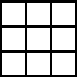
\includegraphics[width=0.15\textwidth]{fig/grid33.pdf}
  }\hspace{1cm}
  \subfloat[4-NH graph]{\label{fig:gg_33_4}
    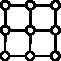
\includegraphics[width=0.15\textwidth]{fig/grid33_4.pdf}
  }\hspace{1cm}
  \subfloat[8-NH graph]{\label{fig:gg_33_8}
    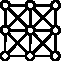
\includegraphics[width=0.15\textwidth]{fig/grid33_8.pdf}
  }
  \end{center}
  \caption{
  An image \Cref{fig:gg_33} can be treated as a grid graph. 
  Two different types of grid graphs can be defined for an image.
  \Cref{fig:gg_33_4} shows a grid graph w.r.t. 4-neighborhood , while
  \cref{fig:gg_33_8} shows a grid graph w.r.t. 8-neighborhood.  
  }\label{fig:grid_graph}
\end{figure}

Many algorithm have been generalized to N-Dimension images.
And since an N-Dimension image itself can be treaded as an \emph{grid graph} or \emph{lattice graph} (see \cref{fig:grid_graph}) any graph based algorithm can be applied to images if they are interpreted as a grid graphs.

Therefore \emph{graph based image analyses} can be viewed as a generalization of \emph{image analyses}.
From a theoretical and  point of view such a generalization is very desirable.
Well studied graph-theoretical approaches as clustering can often directly be applied 
to  \emph{image analyses} \cite{vlachos_1993_csv,arbelaez_2006_cvpr,ohlander_1978_cgip}.

From an algorithmic point of view such a generalization can help to reduce 
code redundancy.
Generic graph algorithm can be written once, and might be applied 
to images (2D, 3D ,3D+t , N-Dimensional Images ) and graphs (grid graphs, 
regions adjacency graphs, nearest neighbor graphs).

In addition, many graph based algorithms are build on top of
very simple building blocks 
as \emph{minimum spanning trees}, \emph{hierarchical clustering} and 
\emph{shortest path algorithms}. 

Providing generic and reusable implementation of these building blocks
would be beneficial for the whole image processing community.
Instead of spending a huge amount of time with writing thousands lines code,
researchers could focus more on research itself.

Furthermore we believe, more researchers would provide their code in a more organized fashion, if 
they could build on top of existing solutions.
Instead of many different project with different build systems and incompatible data structures
the usage of a single framework is desirable.







\begin{figure}
\centering
\subfloat[$8x8$ image]{ \label{fig:make_rag_grid}
    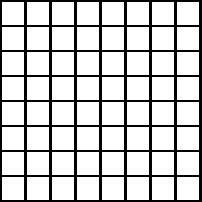
\includegraphics[width=0.25\textwidth]{fig/gridA.pdf}
}
\subfloat[$8x8$ grid graph]{  \label{fig:make_rag_grid_graph}
    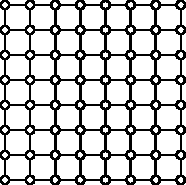
\includegraphics[width=0.25\textwidth]{fig/gridGraphA.pdf}
}
\subfloat[labeled image]{   \label{fig:make_rag_labels_labels}
    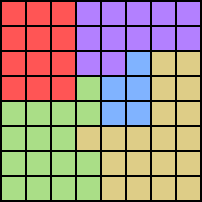
\includegraphics[width=0.25\textwidth]{fig/lgridA.pdf}
}
\\
\subfloat[labeled grid graph]{   \label{fig:make_rag_labels_on_graph}
    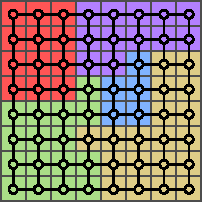
\includegraphics[width=0.25\textwidth]{fig/gridC.pdf}
}
\subfloat[RAG]{     \label{fig:make_rag_rag_a}
    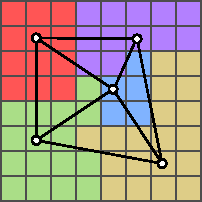
\includegraphics[width=0.25\textwidth]{fig/lgridB.pdf}
}
\subfloat[RAG]{     \label{fig:make_rag_rag_b}
    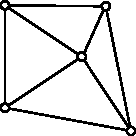
\includegraphics[width=0.25\textwidth]{fig/lgridC.pdf}
}
\caption{
    A labeled grid graph  (\cref{fig:make_rag_grid}, \cref{fig:make_rag_grid_graph}  and \ref{fig:make_rag_labels_labels})
    or any other graph can be turned into an region adjacency graph (\cref{fig:make_rag_labels_on_graph}, \cref{fig:make_rag_rag_a} and \cref{fig:make_rag_rag_b}). 
    Any edge  $\{u,v\}$ where $u$ and $v$ have the same label is contracted and $u$ and $v$ 
    are merged.
}\label{fig:make_rag}
\end{figure}


\section{Contributions}

Within this thesis we make the following contributions:

\begin{compactitem}
    \item We propose and implemented a framework for graph based image analysis 
        build on top of  \emph{vigra} library \cite{software_vigra}. We provide implementations for important graph based algorithms based on the proposed framework.All data structures and algorithm are implemented in fast C++, 
        but can be used from Python for rapid prototyping.
        Ready to use examples are given within this thesis, and will be 
        provided within the branch of \emph{vigra} corresponding to 
        this thesis.



    \item 
        We propose a new algorithm for the multicut objective based on the move
        making paradigm, the \emph{Cut Glue and Cut} algorithm (CGC). We compared the 
        the proposed algorithm on various existing solvers and show
        that CGC outperforms approximative solvers w.r.t. to runtime and still yields
        results very closed to global optimal solutions. We provide an implementation of CGC within the OpenGM framework.



\end{compactitem}


\section{Organization}

This work is organized in the following way.
In \cref{ch:reated_work} related work will be presented and  discussed.



In \cref{ch:cgc} we propose a new algorithm for the multicut objective.
A detailed related work w.r.t. multicuts is given in \cref{sec:gcg_related_work}.
In \cref{sec:experiments} we show an extensive comparison  with existing solvers.



In \cref{ch:vigra_graph_lib} we will propose an implementation of
a graph based framework. 
Design choices will be compared and discussed and most 
important implementation details will be explained.
Ready to use code examples will be given in \cref{ch:the_showcase}.




